%!TEX TS-program = xelatex

\documentclass {beamer}

%\input {inc0gnito.sty}

\useoutertheme{infolines}
\usepackage{ulem}

\usepackage{xetexko}
\usepackage{mathtools}
\usepackage{amsmath}
\usepackage{fontspec}
\usepackage{hyperref}
\usepackage{graphicx}
\usepackage{listings}
\usepackage{makeidx}
\usepackage{indentfirst}
\usepackage{standalone}
\usepackage{tikz}
\usetikzlibrary{positioning,fit,calc}
\tikzset{block/.style={draw, thick, text width=3cm, minimum height=1.5cm, align=center},
% the align command is used to align the block diagram at the center
% the height command adjust the height of the block diagram
% here block diagram refers to the whole diagram, not the single block
% the thick command here signifies the border of all the blocks used inside the block diagram. You can change it to thin command if you want the thin edge of the blocks
line/.style={-latex}   % the lesser the width the greater will be the diagram window
}


%\setmainfont {NanumMyeongjo}
\setsansfont {Noto Sans CJK KR}
\setmainfont {Noto Sans CJK KR}
\setmonofont[Scale=0.8]{DejaVu Sans Mono}

\lstdefinestyle{diff}{
  belowcaptionskip=1\baselineskip,
  breaklines=true,
  frame=L,
  xleftmargin=\parindent,
  showstringspaces=false,
  % Diffstart
  morecomment=[f][\color{gray}]{@@},
  % Diffincl
  morecomment=[f][\color{Green}]{+},
  % Diffrem
  morecomment=[f][\color{Red}]{-},
  basicstyle=\footnotesize\ttfamily,
}

\lstdefinestyle{customtxt}{
  belowcaptionskip=1\baselineskip,
  breaklines=true,
  frame=L,
  xleftmargin=\parindent,
  showstringspaces=false,
  basicstyle=\footnotesize\ttfamily,
}

\lstdefinestyle{customc}{
  belowcaptionskip=1\baselineskip,
  breaklines=true,
  frame=L,
  xleftmargin=\parindent,
  language=C,
  showstringspaces=false,
  basicstyle=\footnotesize\ttfamily,
  keywordstyle=\bfseries\color{green!40!black},
  commentstyle=\itshape\color{purple!40!black},
  identifierstyle=\color{blue},
  stringstyle=\color{orange},
}


\hypersetup {
  colorlinks, linkcolor=blue
}

\title {HTTP / CGI web server \& app proposal}
\author {'); DROP TABLE teams}


\AtBeginSection[]
{
  \begin{frame}
    \frametitle{Index}
    \tableofcontents[currentsection]
  \end{frame}
}

\begin {document}

\begin{frame}
  \titlepage
\end{frame}

\begin{frame}
  \frametitle{0x00 - What is HTTP / CGI?}
  \framesubtitle{TCP 80}

  What is HTTP/1.0 and CGI/1.1?

  \begin{itemize}
    \item<1-> HTTP/1.0: a wishy-washy protocol based on common usage that IESG apparently "has concerns" about.
    \item<2-> CGI/1.1: some dumb Apache memo on making old web apps vulnerable to DDoS attacks.
    \item<3-> Both: Protocols used for stuffs.
    \item<3-> Non-binding, World-Wide Web, lorem ipsum.
  \end{itemize}
\end{frame}

\begin{frame}
  \frametitle{0x01 - Our idea: a HTTP / CGI guest book server}
  \framesubtitle{TCP 80}

  So you can tell your friend you wired them the money.

  \begin{itemize}
    \item<1-> Open to expansion:
    \item<2-> File/FTP server
    \item<3-> \sout{Chat server} IRC server
    \item<4-> Database, webhook...
    \item<5-> ...and many more
  \end{itemize}
\end{frame}

\begin{frame}
  \frametitle{0x02 - Why build a HTTP / CGI guest book server?}
  \framesubtitle{TCP 80}

  Why HTTP/1.0

  \begin{itemize}
    \item<1-> Basic socket programming
    \item<2-> ...but it also requires some parsing, child process management, etc.
    \item<3-> Will be an interesting project to implement
    \item<3-> (we can hide vulnerabilities in creative ways)
  \end{itemize}
\end{frame}

\begin{frame}
  \frametitle{0x02 - Why build a HTTP / CGI guest book server?}
  \framesubtitle{Common Gateway Interface}

  Why CGI/1.1

  \begin{itemize}
    \item<1-> Old-fashioned way to develop web apps
    \item<2-> Use \textit{env vars} and \textit{pipes} to transfer data between client and server
    \item<3-> For demonstration purposes + a way to hide some vulns in it
    \item<4-> Opens up making challenging low-level exploits depending on implementation
  \end{itemize}
\end{frame}

\begin{frame}
  \frametitle{0x03 - Overall architecture}
  \framesubtitle{GNA's Not Apache!}

  \centering
  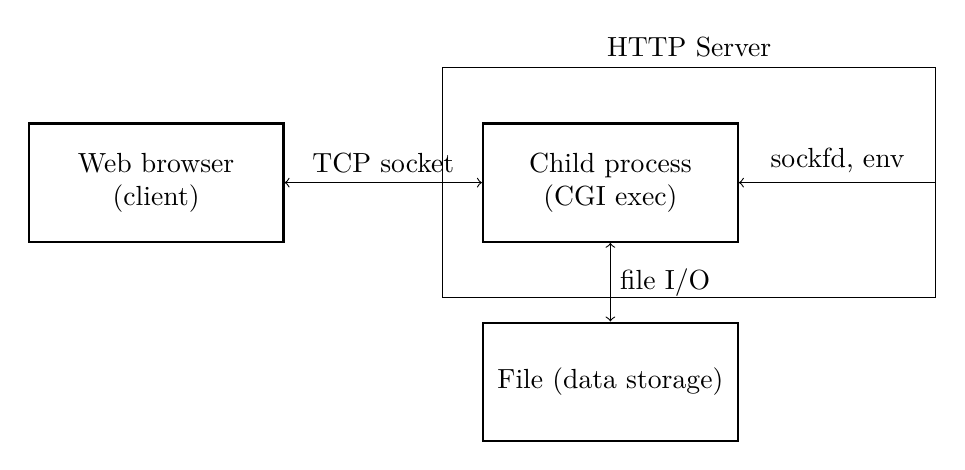
\begin{tikzpicture}
    \node[block] (a) {Child process (CGI exec)};
    \node[block,below=of a] (b) {File (data storage)};
    \node[draw,xshift=10mm,inner xsep=15mm,inner ysep=7mm,fit=(a),label={HTTP Server}](c){};
    \node[block,left=of c,xshift=-10mm] (d) {Web browser (client)};
    \draw[line, <->] (a) -- (b) node[midway,right] {file I/O};
    \draw[line, ->] (c.east) -- (a.east) node[midway,above] {sockfd, env};
    \draw[line, <->] (d) -- (a) node[midway,above] {TCP socket};
  \end{tikzpicture}
\end{frame}

\begin{frame}
  \frametitle{0x04 - Features}
  \framesubtitle{HTTP server}

  Features for the HTTP server

  \begin{itemize}
    \item<1-> We will not implement the whole of RFC 1945 (HTTP/1.0).
    \item<2-> Instead, a \textit{subset} of RFC 1945 barely able to serve the page.
    \item<3-> An original implementation without using any off-the-shelf libraries (planned)
  \end{itemize}
\end{frame}

\begin{frame}
  \frametitle{0x04 - Features}
  \framesubtitle{CGI/1.1 program}

  Features for the CGI

  \begin{itemize}
    \item<1-> Likewise, we will not implement the whole of RFC 3875 (CGI/1.1).
    \item<2-> Instead, a \textit{subset} of RFC 3875 barely able to run our CGI app.
    \item<3-> Again, an original implementation (planned)
  \end{itemize}
\end{frame}

\begin{frame}
  \frametitle{0x04 - Features}
  \framesubtitle{CGI guest book}

  Features for the CGI guest book app
  \begin{itemize}
    \item<1-> Takes user input \textit{\{nickname, message\}} using POST
    \item<2-> Stores given data into a simple TSV/redis-based data storage
    \item<3-> Implements CGI/1.1 \& a basic rendering engine
    \item<3-> libCGI will be used to parse CGI env vars/message-body (planned)
  \end{itemize}
\end{frame}

\begin{frame}
  \frametitle{0x05 - Questions?}
  \framesubtitle{Thank you for listening!}

  Are there any questions?
  \begin{itemize}
    \item<1-> Thank you for your attention.
  \end{itemize}
\end{frame}

\end {document}
